\documentclass[usenames,dvipsnames,8pt,aspectratio=169]{beamer}
\usepackage{amsmath,amsfonts,amssymb}
\usepackage{mathtools}
\usepackage{etex} %for Windows
\usepackage[utf8]{inputenc}
\usepackage[english, russian]{babel} 
%\usepackage{microtype}			% Better interword spacing and additional kerning.
\usepackage{ellipsis}			% Adjusted space with \dots between two words.
\usepackage{graphicx}
\usepackage{pstricks}

\usepackage{xcolor}


\usepackage{changepage}

\usepackage{algorithm}
\usepackage{algpseudocode}
%\usepackage[]{algorithm2e}
%\usepackage{algorithmic}

%\usepackage{tcolorbox}


\usepackage{caption}
\usepackage{subcaption}
%\usepackage{stackengine}


\usepackage{tikz}
\usetikzlibrary{tikzmark,calc}
\usetikzlibrary{positioning, backgrounds}
\usetikzlibrary{arrows, chains, matrix, scopes, patterns, shapes, fit}
\usetikzlibrary{mindmap,trees,shadows}
\usetikzlibrary{decorations.pathreplacing}
%\usetikzlibrary{crypto.symbols}

\usepackage{pgfplots}

\pgfmathdeclarefunction{gauss}{2}{%
	\pgfmathparse{1/(#2*sqrt(2*pi))*exp(-((x-#1)^2)/(2*#2^2))}%
}


\tikzset{
	invisible/.style={opacity=0},
	visible on/.style={alt={#1{}{invisible}}},
	alt/.code args={<#1>#2#3}{%
		\alt<#1>{\pgfkeysalso{#2}}{\pgfkeysalso{#3}} % \pgfkeysalso doesn't change the path
	},
}

\newcommand\strikeout[2][]{%
	\begin{tabular}[b]{@{}c@{}} 
		\makebox(0,0)[cb]{{#1}} \\[-0.2\normalbaselineskip]
		\rlap{\color{Orange}\rule[0.5ex]{\widthof{#2}}{1.5pt}}#2
\end{tabular}}

\newcommand\Fontvi{\fontsize{11}{13.2}\selectfont}

\usepackage{listings} % for C++ code

\usepackage{braket}
%\usepackage[braket, qm]{qcircuit}



\usepackage[T1]{fontenc}
%\usepackage[sfdefault,scaled=.85]{FiraSans}
%\usepackage{newtxsf}
%\usepackage[nomap]{FiraMono}

\usepackage{fontawesome} % for ruble sign




\usefonttheme[onlymath]{serif}
\renewcommand\sfdefault{cmbr}

\renewcommand{\bfdefault}{sb}

\definecolor{CharCoalDark}{RGB}{13, 16, 19}
\definecolor{Orange}{RGB}{255, 165,0}
\definecolor{DarkOrange}{RGB}{255, 165,0}
\definecolor{LightSalmon}{RGB}{255, 160, 122}
\definecolor{LeafGreen}{RGB}{34, 139,  34}
\definecolor{Coral}{RGB}{255, 127, 80}
\definecolor{DarkTurquoise}{RGB}{0, 206, 209}

%\newtheorem{defRus}{Определение}
%\newtheorem{thmRus}{Теорема}
%s\newtheorem{corRus}{Следствие}


\setbeamercolor{background canvas}{bg=CharCoalDark}

\setbeamerfont{title}{series=\bfseries}
\setbeamercolor{title}{fg=Orange}
\setbeamercolor{section in toc}{fg=white}
\setbeamercolor{frametitle}{fg=Orange}
\setbeamercolor{normal text}{fg=white}
%\setbeamercolor{normal text}{fontsize=12pt}
\setbeamercolor{itemize item}{fg=Orange}
\setbeamercolor{enumerate item}{fg=Orange}
\setbeamercolor{enumerate item item}{fg=Orange}
\setbeamercolor{itemize item item}{fg=Orange}
\setbeamercolor{enumerate item}{fg=Orange}
\setbeamercolor{block title}{bg=DarkOrange,fg=white}
\setbeamerfont{block title}{series=\bfseries}

\setbeamertemplate{itemize item}[circle]
\setbeamertemplate{eumerate subitem}{\color{Orange}[$\checkmark$]}
\setbeamertemplate{itemize subitem}{\color{Orange}\Large$\textbullet$}
\setbeamertemplate{itemize subitem}{\color{Orange} \tiny $\blacksquare$}

% footnote without a marker
\newcommand\blfootnote[1]{%
	\begingroup
	\renewcommand\footnoterule{}
	\renewcommand\thefootnote{}\footnote{#1}%
	\addtocounter{footnote}{-1}%
	\endgroup
}

\newcommand*{\Scale}[2][4]{\scalebox{#1}{\ensuremath{#2}}}%

\newcommand\Item[1][]{%
	\ifx\relax#1\relax  \item \else \item[#1] \fi
	\abovedisplayskip=0pt\abovedisplayshortskip=0pt~\vspace*{-\baselineskip}}


\newcommand{\AxisRotator}[1][rotate=0]{%
	\tikz [x=0.45cm,y=1.2cm,line width=.2ex,-stealth,#1] \draw[color=Orange] (0,0) arc (-150:150:2 and 1);%
}

\usepackage[absolute,overlay]{textpos} %to clip to a corner
\newcommand\FrameText[1]{%
	\begin{textblock*}{\paperwidth}(\textwidth-35pt, 10 pt)
		\raggedright #1\hspace{.5em}
\end{textblock*}}

\makeatletter
\let\save@measuring@true\measuring@true
\def\measuring@true{%
	\save@measuring@true
	\def\beamer@sortzero##1{\beamer@ifnextcharospec{\beamer@sortzeroread{##1}}{}}%
	\def\beamer@sortzeroread##1<##2>{}%
	\def\beamer@finalnospec{}%
}
\makeatother

\AtBeginSection[]
{
	\begin{frame}<beamer>
		\frametitle{Outline}
		\tableofcontents[currentsection]
	\end{frame}
}



\titlegraphic{
	
	%\includegraphics[width=2.5cm]{erc_logo_gray}\hspace*{2.5cm}~%
	%\includegraphics[width=4.0cm]{ens_logo_gray}
}
\title{Лекция №4 \\[10pt]
	Коды аутентификации сообщений. \\[5pt]
	Криптографическая хэш-функция}

\date{ Елена Киршанова \\  \textbf{Курс ``Основы криптографии''} \\  }



\setbeamertemplate{navigation symbols}{} %removes navigation

% proper highlightling of a code-snippet
\lstset{language=C++,
	keywordstyle=\color{magenta},
	stringstyle=\color{Goldenrod},
	commentstyle=\color{gray},
	breaklines=false,
	%morecomment=[l][\color{magenta}]{\#}
}

%\setlength{\parskip}{8pt}
% ==================================================================
% Definitions for this paper
% ==================================================================
\mathchardef\hyphen="2D

\usepackage{multirow}
\usepackage{multicol} % For multiple coloumn environments
%\usepackage{stmaryrd} % For set brackets
% \setlength{\columnsep}{15pt} % Defining the coloumn seperation
% \setlength{\columnseprule}{1pt} % Place a line between coloumns
% \newcommand{\tab}{\hspace*{2em}}

%subscripts

\newcommand*\SmallTextScript[2]{{\mathchoice{\displaystyle #2}
		{\textstyle #2}%dito
		{\scalebox{#1}{\ensuremath{\scriptstyle #2}}}%
		{\scalebox{#1}{\ensuremath{\scriptscriptstyle #2}}}%
}}


% ADVERSARIES AND SUCH
\newcommand*{\poly}{\ensuremath{\mathrm{poly}}}
\newcommand*{\eps}{\ensuremath{\varepsilon}}
\newcommand*{\alg}{\ensuremath{\mathcal{A}}}

% GROUPS/DISTRIBUTIONS/SETS/LISTS
\newcommand{\N}{{{\mathbb N}}}
\newcommand{\Z}{{{\mathbb Z}}}
\newcommand*{\IZ}{\ensuremath{\mathbb{Z}}}
\newcommand*{\IN}{\ensuremath{\mathbb{N}}}
\newcommand*{\IQ}{\ensuremath{\mathbb{Q}}}
\newcommand{\R}{{{\mathbb R}}}
\newcommand*{\IR}{{{\mathbb R}}}
\newcommand{\Zp}{\ints_p} % Integers modulo p
\newcommand{\Zq}{\ints_q} % Integers modulo q
\newcommand{\Zn}{\ints_N} % Integers modulo N
\newcommand{\F}{\ensuremath{\mathbb{F}}}
\newcommand{\CC}{\ensuremath{\mathbb{C}}}

\newcommand{\GF}{\ensuremath{\mathbb{F}_2}}
\newcommand{\GFn}{\ensuremath{\mathbb{F}^n_2}}

%%% ALGORITHMS/PROCEDURES %%%
\newcommand{\Dec}{\textsf{Dec}}
\newcommand{\Enc}{\textsf{Enc}}
\newcommand{\KeyGen}{\textsf{KeyGen}}
\newcommand{\Gen}{\textsf{Gen}}
\newcommand{\sk}{\textsf{sk}}
\newcommand{\pk}{\textsf{pk}}
\newcommand{\vk}{\textsf{vk}}
\newcommand{\mesS}{\ensuremath{\mathcal{M}}}
\newcommand{\keyS}{\ensuremath{\mathcal{K}}}
\newcommand{\cipS}{\ensuremath{\mathcal{C}}}
\newcommand{\tagS}{\ensuremath{\mathcal{T}}}
\newcommand{\mactag}{\textsf{tag}}
\newcommand{\Hash}{\ensuremath{\mathcal{H}}}
\newcommand{\EID}{\ensuremath{\mathtt{EphID}}}


\newcommand{\adv}{\ensuremath{\mathcal{A}}}

\newcommand{\LWE}{\mathsf{LWE}}
\newcommand{\DCP}{\mathsf{DCP}}
\newcommand{\EDCP}{\mathsf{EDCP}}
\newcommand{\UEDCP}{\mathsf{U \text{-} EDCP}}
\newcommand{\GEDCP}{\mathsf{G \text{-} EDCP}}



%% Landau and proba
\newcommand{\bigO}{\mathcal{O}}
\newcommand*{\OLandau}{\bigO}
\newcommand*{\WLandau}{\Omega}
\newcommand*{\xOLandau}{\widetilde{\OLandau}}
\newcommand*{\xWLandau}{\widetilde{\WLandau}}
\newcommand*{\TLandau}{\Theta}
\newcommand*{\xTLandau}{\widetilde{\TLandau}}
\newcommand{\smallo}{o} %technically, an omicron
\newcommand{\wLandau}{\omega}
\newcommand{\negl}{\mathrm{negl}}
\newcommand*\PROB\Pr 
\DeclareMathOperator*{\EXPECT}{\mathbb{E}}
\DeclareMathOperator*{\VARIANCE}{\mathbb{V}}
\DeclareMathOperator*{\LOGBIAS}{\mathbb{LB}}

\newcommand{\supp}{\ensuremath{\mathsf{sup}}}
\newcommand{\Distr}{\ensuremath{\mathcal{D}}}

% Lattices

% \newcommand{\coset}{\Lambda} % Lambda Lattice
% \newcommand{\cosetPerp}{\Lambda^{\bot}} % Lambda_Perp Lattice
% \newcommand{\gadget}{\textbf{G}} %Gaget matrix
% \newcommand{\mes}{\textbf{m}} %message vector
% \newcommand{\AMat}{\textbf{A}} %A matrices
% \newcommand{\BMat}{\textbf{B}} %B matrices
% \newcommand{\RMat}{\textbf{R}} %R matrices
% \newcommand{\HMat}{\textbf{H}} %H matrices
% \newcommand{\XMat}{\textbf{X}} %H matrices
% \newcommand{\mbar}{\bar{m}} %mBar dimension
% % \newcommand{\gauss}{\mathcal{D}} % gaussian distribution
% \newcommand{\Id}{\textbf{I}} % Identity matrix
% \newcommand{\er}{\textbf{e}} % gaussian distr. vectors
% % \newcommand{\cipher}{\textit{c}} % ciphertext
% \newcommand{\Olwe}{\mathcal{O}_{\textsf{LWE}}} %LWE oracle
% \newcommand{\OSample}{\mathcal{O}_{Sample}} %LWE oracle
% \newcommand{\SigmaB}{\boldsymbol{\Sigma}} %semi-deifinite matrix Sigma%
% % \newcommand{\mods}{\text{ mod}}


%Vectors and Matrices

\newcommand{\AMat}{\mathbf{A}} %A matrices
\newcommand{\BMat}{\mathbf{B}} %B matrices
\newcommand{\DMat}{\mathbf{D}} %Diagonal


\newcommand{\HMat}{\ensuremath{\mathbf{H}}}
\newcommand{\QMat}{\ensuremath{\mathbf{Q}}}
\newcommand{\Id}{\ensuremath{\mathbf{I}}}
\newcommand{\ZeroM}{\textbf{0}} % Zero matrix

\newcommand{\avec}{\ensuremath{\mathbf{a}}}
\newcommand{\bvec}{\ensuremath{\mathbf{b}}}
\newcommand{\cvec}{\ensuremath{\mathbf{c}}}
\newcommand{\evec}{\ensuremath{\mathbf{e}}}
\newcommand{\rvec}{\ensuremath{\mathbf{r}}}
\newcommand{\svec}{\ensuremath{\mathbf{s}}}
\newcommand{\tvec}{\ensuremath{\mathbf{t}}}
\newcommand{\vvec}{\ensuremath{\mathbf{v}}}
\newcommand{\zvec}{\ensuremath{\mathbf{z}}}
\newcommand{\xvec}{\ensuremath{\mathbf{x}}}
\newcommand{\yvec}{\ensuremath{\mathbf{y}}}
\newcommand{\uvec}{\ensuremath{\mathbf{u}}}
\newcommand{\zerovec}{\ensuremath{\mathbf{0}}}

\newcommand{\nth}{^{\mathrm{th}}}
\newcommand{\nd}{^{\mathrm{nd}}}

\newcommand{\RepMMT}{\ensuremath{\mathcal{R}_{\protect\SmallTextScript{0.70}{\texttt{MMT}}}}}
\newcommand{\RepBJMM}{\ensuremath{\mathcal{R}_{\protect\SmallTextScript{0.70}{\texttt{BJMM}}}}}
\newcommand{\XOR}{\ensuremath{\mathtt{3XOR}}}


% % % % % \newcommand{\mb}[1]{\mathbf{#1}} % does not compile otherwise
%%% Removed by Gotti; this is just asking to screw up with packages that (properly) define \mb (mathbold)

% \newcommand{\bL}{\|\bvec_1\|} % b1 length that appears way too often
% \newcommand{\dL}{\|\dvec_1\|} % b1 length that appears way too oftend

%Norms and Scalar products

\newcommand*\abs[1]{\left\lvert#1\right\rvert}
\newcommand*\norm[1]{\left\lVert#1\right\rVert}
\newcommand*\normalabs[1]{\lvert#1\rvert} 
\newcommand*\normalnorm[1]{\lVert#1\rVert}
\newcommand*\bignorm[1]{\bigl\lVert#1\bigr\rVert}
\newcommand*\bigabs[1]{\bigl\lvert#1\bigr\rvert}
\newcommand*\Bigabs[1]{\Bigl\lvert#1\Bigr\rvert}
\newcommand*{\ScProd}[2]{\ensuremath{\langle#1\mathbin{,}#2\rangle}} %Scalar Product
% \newcommand*{\ScProd}[2]{\ensuremath{\langle#1 \:{,}\:#2\rangle}} %Scalar Product
\newcommand*{\bigScProd}[2]{\ensuremath{\bigl\langle#1\mathbin{,}#2\bigr\rangle}} %Scalar Product
\newcommand*{\BigScProd}[2]{\ensuremath{\Bigl\langle#1\mathbin{,}#2\Bigr\rangle}} %Scalar Product
\newcommand{\dist}{\ensuremath{\text{dist}}}


%Some other math operators

\DeclareMathOperator{\Span}{Span} %span of vectors
\DeclareMathOperator{\vol}{\mathrm{vol}} %volume
\DeclareMathOperator{\LW}{LambertW} %Lambert W function
\DeclareMathOperator{\SD}{SD}
\DeclareMathOperator{\gradient}{grad}
\DeclareMathOperator{\TRACE}{Tr}
\newcommand*{\dDR}{\mathrm{d}} %de-Rham-Differential (the d in dx, dy, dz and so on)


%Lists
\renewcommand{\L}{\ensuremath{\mathcal{L}}}

\renewcommand{\P}{\ensuremath{\mathcal{P}}}

\newcommand*{\Lout}{\ensuremath{\L_{\mkern-0.5mu\protect\SmallTextScript{0.85}{\textup{out}}}}}
\newcommand*{\Sout}{\ensuremath{S_{\mkern-0.5mu\protect\SmallTextScript{0.85}{\textup{out}}}}}
\newcommand{\wt}{\ensuremath{\mathit{wt}}}


\newcommand*{\softO}{\widetilde{\bigO}}

\newcommand{\const}{\mathsf{c}} 


\newcommand{\transpose}{\mkern0.7mu^{\mathsf{ t}}}

%proper overline reduced by 1.5mu
\newcommand{\overbar}[1]{\mkern 1.5mu\overline{\mkern-1.5mu#1\mkern-1.5mu}\mkern 1.5mu}

\DeclareMathOperator{\erf}{erf} %error function
\DeclareMathOperator{\erfc}{erfc} %complementary error function
\newcommand{\Er}{\ensuremath{\mathrm{Er}}} %complementary error function


% LATTICES

\newcommand{\Lat}{\ensuremath{\mathcal{L}}}
\newcommand*{\Sphere}[1]{\ensuremath{\mathsf{S}^{#1}}}
%\DeclareMathOperator{\Conf}{Conf}
\newcommand{\Conf}{\mathcal{C}}

%Thick line for table
\setlength{\doublerulesep}{0pt}
\newcommand{\thickline}{\hline\hline\hline}


%circled text
\newcommand*\circled[1]{\tikz[baseline=(char.base)]{
    \node[shape=circle,draw,inner sep=0.3 pt] (char) {\scriptsize #1};}}


%Fix Algorithmicx package
\def\NoNumber#1{{\def\alglinenumber##1{}\State #1}\addtocounter{ALG@line}{-1}}

%For comments
\newcommand{\GColor}{ForestGreen}  %Damiens' color
\newcommand{\EColor}{MidnightBlue} %Elena's color

\newcommand*{\E}[1]{{\color{\EColor} #1} } 
\newcommand*{\G}[1]{{\color{\GColor} #1} } 

%Proper limit with the subscript underneath
% \newcommand{\Lim}[1]{\raisebox{0.5ex}{\scalebox{0.8}{$\displaystyle \lim_{#1}\;$}}}


%TIKZ dense dotted pattern

\pgfdeclarepatternformonly{my dots}{\pgfqpoint{-1pt}{-1pt}}{\pgfqpoint{2.0pt}{2.0pt}}{\pgfqpoint{2pt}{2pt}}%
{
	\pgfpathcircle{\pgfqpoint{0pt}{0pt}}{.35pt}
	\pgfpathcircle{\pgfqpoint{1pt}{1pt}}{.35pt}
	\pgfusepath{fill}
}


\tikzset{
	master/.style={
		execute at end picture={
			\coordinate (lower right) at (current bounding box.south east);
			\coordinate (upper left) at (current bounding box.north west);
		}
	},
	slave/.style={
		execute at end picture={
			\pgfresetboundingbox
			\path  (lower right)rectangle (upper left) ;
		}
	}
} %all defs
\begin{document}
	
\begin{frame}
	\titlepage
\end{frame}


\begin{frame}{Конфиденциальность \& целостность}
\LARGE 

\begin{itemize}
	\itemsep 1em
	\item В предыдущих лекциях: {\color{Orange} конфиденциальность} сообщений
	\item В этой лекции:  {\color{Orange} целостность}
\end{itemize}

\vspace{20pt}
\LARGE {\color{Orange}Криптопрититив}: Код Аутентификации Сообщения (или Имитовставка)  \\[5pt] 
Message Authentication Code (MAC) 


\end{frame}

\begin{frame}{Мотивация}
\Large
	\begin{center}
		\begin{tabular}{c c c c c}
			& Алиса  & & Боб &  \\
			& \multirow{5}{*}{
\includegraphics[scale=0.15]{Alice}} & &
			\multirow{5}{*}{
\includegraphics[scale=0.15]{Bob}} &  \\
			&  & \Huge $\xrightarrow{\text{``Переслать \texttt{1000 \faRub } на карту XXXX'' }}$ & &  \\[20pt]
			\multicolumn{5}{c}{
\includegraphics[scale=0.15]{Eve}} \\
			\multicolumn{5}{c}{Ева}
		\end{tabular}
	\end{center}

	
\end{frame}


\begin{frame}{MAC: определение}
\Large
Цель: отправить сообщение $m$ от Алису к Бобу так, что бы злоумышленник не смог модифицировать $m$, оставаясь незамеченным \\[10pt]
\begin{center}
	\begin{tabular}{c c c c c}
		& Alice  & & Bob &  \\
		& \multirow{5}{*}{
\includegraphics[scale=0.18]{Alice}} & &
		\multirow{5}{*}{
\includegraphics[scale=0.18]{Bob}} &  \\
		&  & \Huge $\xrightarrow{\mkern25mu m, \; \mactag \mkern25mu}$ & &  \\ 
		\LARGE $k \in \keyS$ &   & &  & $k \in \keyS$ \\[10pt]
		$\mactag \leftarrow S(k,m)$   & & &  &    \\ [20pt] 
		\multicolumn{5}{r}{$V(k,m, \mactag) \in \{ 0, 1\}$ }  \\
	\end{tabular}
\end{center}
\pause
\large
{\color{Orange} Код Аутентификации Сообщения } состоит из 3-х ppt алгоритмов:
\vspace{-2pt}
\begin{itemize}
	\item Генерация ключа: $\KeyGen(1^\lambda): k \leftarrow \keyS$ \\[4pt]
	\item Генерация тага: $S(k, m): \mactag \leftarrow \tagS$ \\[4pt]
	\item Верификация тага: $V(k, m, \mactag): \{0, 1\}  $
\end{itemize}
\end{frame}

\begin{frame}{MAC: корректность и безопасность}
\Large
{\color{Orange} Код Аутентификации Сообщения } состоит из 3-х ppt алгоритмов:
\vspace{-2pt}
\begin{itemize}
	\item Генерация ключа: $\KeyGen(1^\lambda): k \leftarrow \keyS$ \\[4pt]
	\item Генерация тага: $S(k, m): \mactag \leftarrow \tagS$ \\[4pt]
	\item Верификация тага: $V(k, m, \mactag): \{0, 1\}  $
\end{itemize}

\vspace{10pt}
{\color{Orange} Корректность:} \LARGE 
$ V(k, m, S(k,m)) = 1 \; \forall \; m \in \mesS, k \in \keyS $

\vspace{10pt}
{\color{Orange}Безопасность:}
Для ppt атакующего $\adv$, имеющего пары $\{(m_1, t_1), \ldots, (m_N, t_N) \}$ для $m_i$, выбранных им самим, $\adv$ не может сгенерировать новую пару  $(m,t)$
\[(m,t) \notin \{(m_1, t_1), \ldots, (m_N, t_N) \}\]

\vspace{10pt}

Поэтому безопасная длина тага: $96, 128, 256 $ бит.
\end{frame}

\begin{frame}{MAC: безопасность}

\Large 
\begin{center}
	$I = (\KeyGen, S, V)$ --  MAC \\[10pt]
	
	\begin{tabular}{c c c}
		{\color{Orange} Челленджер $\mathcal{C}$ } & & {\color{Orange} Атакующий $\mathcal{A}$ }\\ [5pt]
		$k \leftarrow \KeyGen(1^\lambda)$ & $\xrightarrow{\quad \lambda \quad}$  &\\[5pt]
		& $\xleftarrow{\quad  m_i \quad}$  &$m_i\leftarrow \mesS $\\ [5pt]
		
		$t_i \leftarrow S(k, m_i)$ & $\xrightarrow{\quad t_i \quad}$ &\\ [5pt]

		& $\xleftarrow{\quad  (m^\star, t^\star) \quad}$ & \\ [5pt]
	\end{tabular}
	\begin{tikzpicture}[overlay]
	%\draw[fill=none, draw=white, opacity=0.5] (-8.5,-2.3) rectangle (-5.0,2.7); 
	%\draw[fill=none, draw=white, opacity=0.5] (-3.0,-2.3) rectangle (0.0,2.7); 
	\end{tikzpicture}
\end{center}

\vspace{5pt}
$\mathtt{W_{I, \adv}}$ -- событие $Ver(k, m^\star, t^\star) == 1$. \\ [4pt]
$\mathtt{MacAdv} = \Pr[\mathtt{W_{I, \adv}}] $ -- выигрыш  $\adv$. \\ [4pt]
\color{Orange} Схема MAC $I$ безопасна, если для любого ppt $\adv:$  \[\mathtt{MacAdv} = \negl(\lambda).\]
\end{frame}


\begin{frame}{Конструкции MAC}
\Large
\begin{enumerate}
	\itemsep1em
	\item Блок-шифр  (AES, ГОСТ), псевдослучайная ф-ия $f$  -- примеры конструкции MAC для 16-байтных сообщений
	\begin{align*}
			S(m) &:= f(k, m) \rightarrow t \\
			V(k, m, t) & :=f(k, m) == t \; ? \;  1 : 0 
	\end{align*}

	
	\item Для более длинных сообщений:  \\[10pt]
		-- CBC-MAC (целостность банковских транзакций) \\ 
		Стандарты: ANSI, FIPS 186-3, ГОСТ \\[5pt]
		-- NMAC (Nested MAC) \\[5pt]
		-- HMAC (SSL, IPSec)
\end{enumerate}

\end{frame}

\begin{frame}{ECBC-MAC }
\Large
 $m = (m_1, m_2, m_3, ...)$, $\textbf{F}-$ блок-шифр (AES, ГОСТ), $|m_i|$  --  128 бит
	\begin{figure}
		\includegraphics[width=0.75\textwidth]{CBC_MAC}
	\end{figure}
\vspace{-90pt}

\Large 
$V((k, k1), m)$ выполняет идентичные шаги.\\[10pt]

Отличия от CBC-mode:
\begin{itemize}
	\itemsep 5pt
	\item $k, k1$ - два {\color{Orange} разных} ключа для $\textbf{F}$
	\item Не используется IV
	\item Выходное значение \textbf{tag} может быть урезано (тем самым уменьшая безопасность схемы, стандарты ANSI X9.19, ISO/IEC 9797)
\end{itemize}

\end{frame}


\begin{frame}{Вложенный (Nested) MAC}
	\Large
	\vspace{-25pt}
	$m = (m_1, m_2, m_3, ...)$, $\textbf{F}-$ блок-шифр (AES, ГОСТ), $|m_i|$ -- $n$ бит, $k  \in \{0,1\}^\kappa$.
	\begin{figure}
		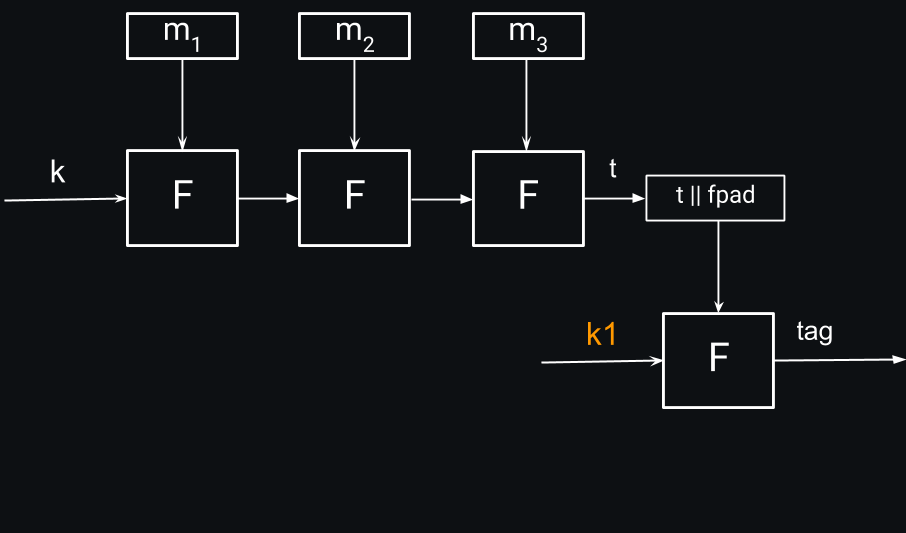
\includegraphics[width=0.75\textwidth]{NMAC}
	\end{figure}
\vspace{-40pt}
$
	\text{fpad} \in \{0,1\}^{n - \kappa} -\text{любое фиксированное значение}
$
\end{frame}

\begin{frame}{Набивка (padding)}
\Large
\begin{center}
Что если $\mathbf{m} = (m_1, m_2, ...)$ не кратно длине блока?
\end{center}
Пример {\color{Orange} плохой} набивки : добивать $0'$-ми.
\[m = (\star \star \star  ), \quad |m|< 128 \text{бит}\] 

Набивка такого $m$:
\[m_{\text{padded}}=(\star \star \star  \; 0 \ldots 0  ). \] 

Тогда для сообщения $m' = (m||0)$:
\[S(k,m_{\text{padded}}) = S(k, m')\]

\vspace{10pt}
\centering
Для $\mathbf{m} \neq \mathbf{m'}$, должно выполнятся $\mathbf{m}||\text{pad} \neq \mathbf{m'}||\text{pad}$. \\[5pt]
 Набивка должна быть функцией $1 \leftrightarrow 1$.
	
\end{frame}

\begin{frame}{Набивка (padding)}
	\Large
	\begin{enumerate}
		\itemsep1em
		\item {\color{Orange} ISO.} Набивка: $10\ldots0$. `1' означает начало набивки. \\
		Добавляется фиктивный блок, если $|m| < $ длина блока
		\item {\color{Orange} NIST, GOST}  
		\begin{figure}
			\captionsetup[subfigure]{labelformat=empty}
			\begin{subfigure}{.5\textwidth}
				\hspace{-30pt}
				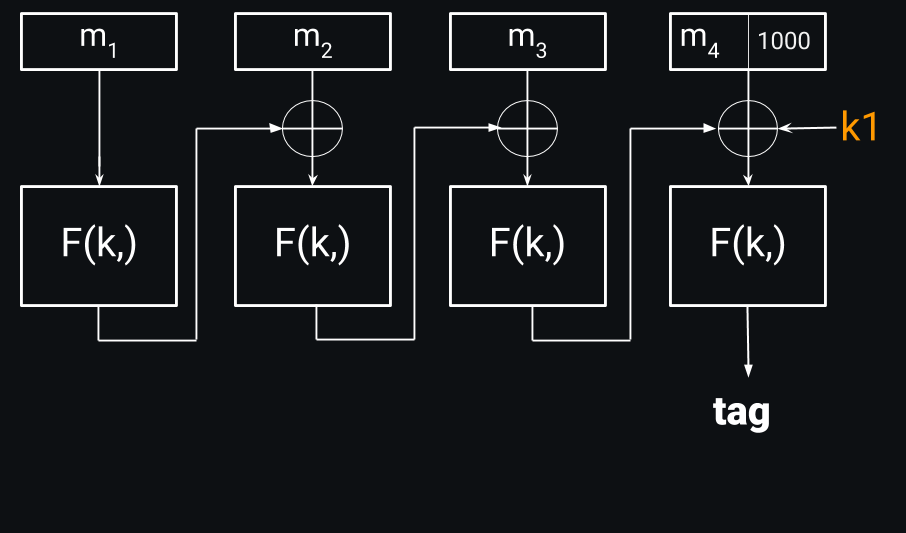
\includegraphics[width=.95\textwidth]{CBC_Mac_Padding}
				\caption{\hspace{-30pt}  \Large $m_4$< длина блока}
			\end{subfigure}%
		 \begin{subfigure}{.5\textwidth}
		\hspace{-36pt}
			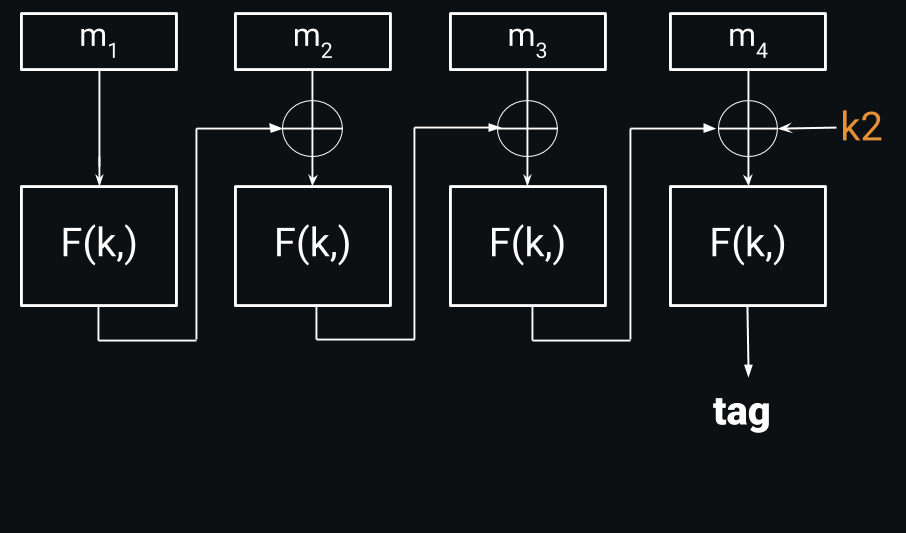
\includegraphics[width=.95\textwidth]{CBC_Mac_Padding_1}
			\caption{\hspace{-50pt}  \Large $m_4$= длина блока}
		\end{subfigure}%
		\end{figure}
		\vspace{1em}
		Преимущества: нет фиктивного блока, нет дополнительного вызова F.
		 
	\end{enumerate}
\end{frame}


\begin{frame}{Двухфакторная аутентификация}

\Large 
Двухфакторная аутентификация = пользователь предоставляет то, что он {\color{Orange} знает} (пароль) + то, чем он {\color{Orange} владеет} (смартфон) 

\[
I = (\KeyGen, S, V) - \text{ MAC }  
\]

\vspace{10pt}
%	\begin{center}
	\begin{tabular}{c c c c c}
		 Пользователь &  & &  & Сервер \\
		 \multirow{5}{*}{
\includegraphics[scale=0.12]{Alice}} & & &
		 & \multirow{5}{*}{
\includegraphics[scale=0.12]{Bob}}  \\
		&  $k \leftarrow \KeyGen()$ &  & &  \\
		&  &  $\xrightarrow{ \quad k \quad}$ & &  \\[10pt]
		&  $p = S(k, T)$ &  & &  \\
		& {\small $T$ -- текущая дата, время} & $\xrightarrow{ \quad p \quad}$   & &  \\
		& &  &  & $V(k, p, T)$ \\
	\end{tabular}

\vspace{10pt}
$p$ -- временной одноразовый пароль (timed one-time password).
%\end{center}

\end{frame}

\begin{frame}
Часть II \\ [10pt]
\begin{LARGE}
	
	\color{Orange}
	\Huge Криптографическая хэш-функция
	
\end{LARGE}
\end{frame}

\begin{frame}{Хэш-функции}

\Large
\begin{center}
	{\color{Orange} Криптографическая хэш-функция ! = Хэш-функция} \\[10pt]
\end{center}

Фильтры Блума, контрольные суммы (sumXXX, fletcherXXX),  не являются криптографическими хэш-функциями.


\end{frame}

\begin{frame}{Криптографическая хэш-функция: определение}
\Large
{\color{Orange}Криптографическая хэш-функция} -- \underline{двойка} полиномиальных алгоритмов $(\Gen, \Hash)$:
\begin{enumerate}
\itemsep 7pt
\item Вероятностный $\Gen: s \leftarrow \Gen(1^\lambda)$  
\item Детерминированный $\Hash_s: \{0,1\}^\star \rightarrow \{0,1\}^\ell$,
\end{enumerate}

где $\Hash_s$ является  {\color{Orange} стойкой к коллизиям}: \\[5pt]

для заданного $s$,  не существует ppt алгоритма, который находит $x, x' (x!=x')$,
\[
\Hash_s(x) = \Hash(x')
\]

{\color{Orange} Криптографическая} хэш-функция \underline{обязана} быть стойкой к коллизиям.\\[5pt]

Существует  \underline{много} коллизий для $\Hash_s$, но должно быть \underline{трудно} найти \\ любую коллизию.
\end{frame}

\begin{frame}{Свойство криптографической хэш-функции}
\Large 
\[
\Hash_s: \{0,1\}^\star \rightarrow \{0,1\}^\ell
\]

{\color{Orange} I.} Стойкость к нахождению прообраза (или односторонность) \\[5pt]
Дано: $(s, y \in \{0,1\}^\ell)$\\
Найти: $x$, такой что \ $\Hash_s(x) =  y$ \\[5pt]
{\color{Orange} Стойкая к коллизиям хэш-функция является стойкой к нахождению прообраза}


\vspace{20pt}
{\color{Orange} II.} Стойкость к нахождению $2$-го прообраза \\[5pt]
Дано: $(s, x)$\\
Найти: $x'!=x$, такой что\ $\Hash_s(x) =  \Hash_s(x')$ \\[5pt]
{\color{Orange}  Стойкая к коллизиям хэш-функция является стойкой к нахождению \\ $2$-го прообраза}

\vspace{20pt}

Стойкость к коллизиям  $\implies$ 	{\color{Orange} II.}  $\implies$ 	{\color{Orange} I.}  
\end{frame}

\begin{frame}{Экзотические свойства хэш-функций}
\LARGE
В мире Bitcoin три свойства хэш-функции могу называться иначе:

\begin{align*}
\text{нахождение прообраза} & \rightarrow  \text{``hiding''} \\
\text{нахождение 2-го прообраза} & \rightarrow  \text{``puzzle-friendliness''} \\
\text{стойкость к коллизиям} & \rightarrow  \text{``collision resistance''} \\
\end{align*}


То есть для реализации Bitcoin подойдет криптографическая хэш-функция.

\end{frame}

\begin{frame}{Атака на любую хэш-функцию: парадокс Дней рождений}
\large 
Положим $h_1, h_2, \ldots, h_n \in \{0,1\}^\ell$ независимо случайное выбранные строки. Парадокс Дней рождений
\[
\text{Для } n = \bigO\left (\sqrt{ \abs{ \{0,1\}^\ell }} \right) = \bigO\left( 2^{\ell/2} \right) \quad  \Pr[\exists (i != j) \; : \; h_i = h_j] > 1/2.
\]

Алгоритм перебора находит коллизию после {\color{Orange} $\bigO(2^{\ell/2})$ } вычисленных хэшей: \\
\begin{enumerate}
\itemsep 10pt
\item Выбрать $ 2^{\ell/2}$ случайных строк $m_1, \ldots, m_{2^{\ell/2}}$ 
\item  Для каждой $m_i$ вычислить $h_i = \Hash_s(m_i)$, отсортировать пары $(h_i, m_i)$ по значению\ $h_i$
\item  Найти в упорядоченном списке $h_i = h_j$. Коллизия: $(m_i, m_j)$.
\end{enumerate}			

\vspace{10pt}

Алгоритм успешен с константной вероятностью по парадоксу ДР.
\vfill
\LARGE
{\color{Orange} Вывод:} Требуем  $\ell \geq 160$.
\end{frame}


\begin{frame}{Хэш-функции: исторический дайджест}
\large
\begin{enumerate}
\itemsep7pt
\item 1980e: MD4 (Message Digest) предложено R. Rivest.  {\color{Orange} $\ell = 128$} \\
Статус: {\color{Orange} Взломана.} Коллизию можно найти в течение секунд

\item 1990: MD5. {\color{Orange} $\ell = 128$} \\
Статус: {\color{Orange} Взломана.} Коллизию можно найти в течение секунд
\pause
\item 1995: SHA-1 (Secure Hash Algorithm 1) {\color{Orange} $\ell = 160$ } \\
Статус: {\color{Orange} Взломана}. См.\ \url{https://shattered.io/} два PDF файла с одинаковым значением SHA-1. \\
{\color{Orange} !:} всё еще используется некоторыми системами (GIT).
\pause
\item 2001: SHA-2 (SHA-256, SHA-384, SHA-512). {\color{Orange} $\ell=256, 348, 512$} \\
Статус: {\color{Orange} Считается безопасной.}
\pause
\item 2012: SHA-3 (Keccak). SHA-3 {\color{Orange} $\ell = 224/256/348/512$.} \\
Статус: {\color{Orange} Считается безопасной.} 
\end{enumerate}
\pause
В России:

\begin{enumerate}
\item GOST R 34.11-94 and GOST 34.311-95. {\color{Orange} $\ell = 256$} \\
Статус: {\color{Orange} Считается устаревшей.} Коллизия за $2^{105}$ операций,
\item  GOST R 34.11-2012. Стрибог {\color{Orange} $\ell = 256, 512$} \\
Статус: {\color{Orange} Считается безопасной.}  
\end{enumerate}
\end{frame}

\begin{frame}
Часть III \\ [10pt]
\begin{LARGE}
	
	\color{Orange}
	\Huge Конструкция Меркла-Дамгора
	
\end{LARGE}
\end{frame}

\begin{frame}{Конструкция хэш-функций: парадигма Merkle-Damg\aa rd}
\Large
Из функции компрессии (определим позже) \[h: \keyS \times \mesS \rightarrow \keyS\]
построим $\Hash: \mesS^\star \rightarrow \keyS.$ \\[10pt]

Пусть $m = (m_1, m_2, m_3 )$ произвольной длины
\begin{figure}
	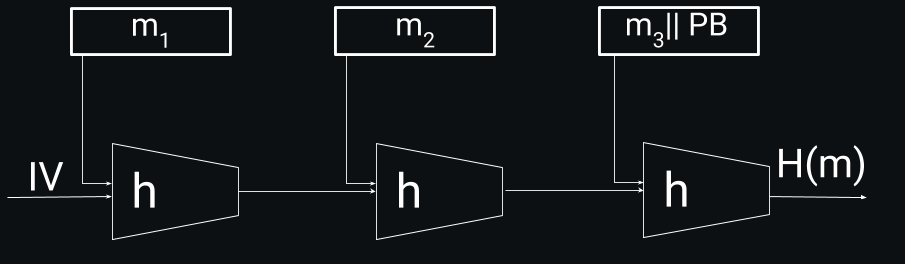
\includegraphics[width=0.8\textwidth]{MerkleDamgard}
\end{figure}

\textbf{IV} -- Начальное значение, фиксировано для конкретной хэш-функции \\
\textbf{PB} -- Блок добивки $\left[100\ldots0 || \; |m|  \; \right]$. \\
Если \textbf{PB}  не влезает, добавляем новый блок.

\end{frame}

\begin{frame}{Безопасность конструкции Merkle-Damg\aa rd}
\Large

\begin{columns}[T]
\begin{column}{0.5\textwidth}
	{\color{Orange} Теорема:} Если $h$ стойкая к коллизиям, то и  $H$ стойкая к коллизиям.
\end{column}
\begin{column}{0.5\textwidth}
	\begin{figure}
		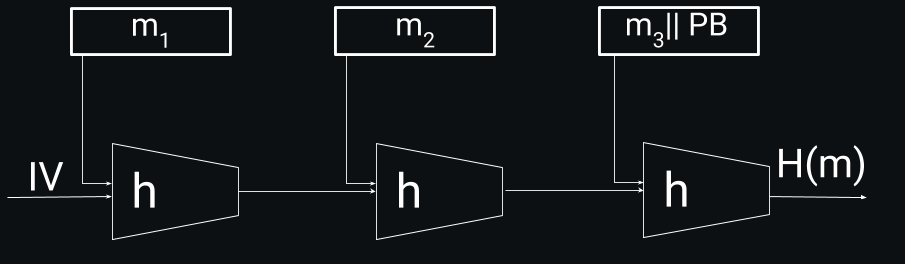
\includegraphics[width=\textwidth]{MerkleDamgard}
	\end{figure}
\end{column}
\end{columns}




\end{frame}

\begin{frame}{Конструкции функции компрессии $h$}
\Large
\[
\Enc: \keyS \times \{0,1\}^n \rightarrow  \{0,1\}^n -\text{блок-шифр.} 
\]

\vspace{10pt}	

{\color{Orange} Конструкция Davies-Meyer:} $	h(H_{i}, m) = \Enc(H_i, m)\oplus H_i .$

\begin{figure}
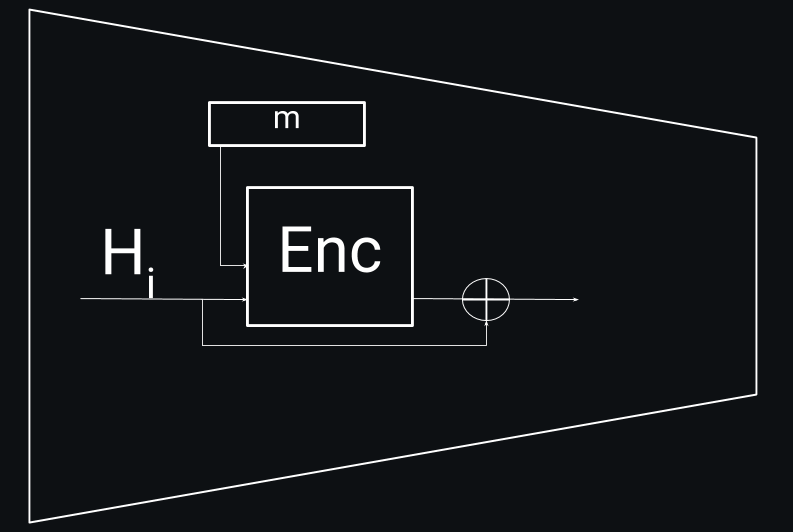
\includegraphics[width=0.6\textwidth]{DaviesMeyerCompression}
\end{figure}
\end{frame}


\begin{frame}{Пример: Функция компрессии в SHA-256}
\Large 

\begin{figure}
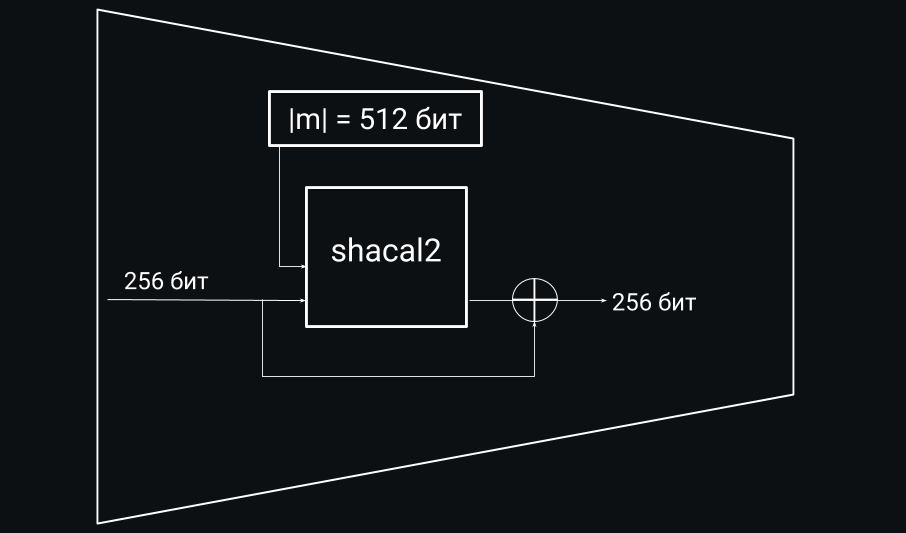
\includegraphics[width=0.8\textwidth]{SHA256}
\end{figure}

\end{frame}

\begin{frame}{Безопасность Davies-Meyer}

\LARGE
\begin{columns}[T]
\begin{column}{0.6\textwidth}
{\color{Orange} Теорема (неформально):}  $\Enc(k, \cdot): \{0,1\}^n \rightarrow \{0,1\}^n$ неотличима от случайной перестановки, то нахождение коллизии $h(H, m) = h(H', m')$ требует $\bigO(2^{n/2})$ вычислений $(\Enc, \Enc^{-1})$.
\end{column}
\begin{column}{0.4\textwidth}
\begin{figure}
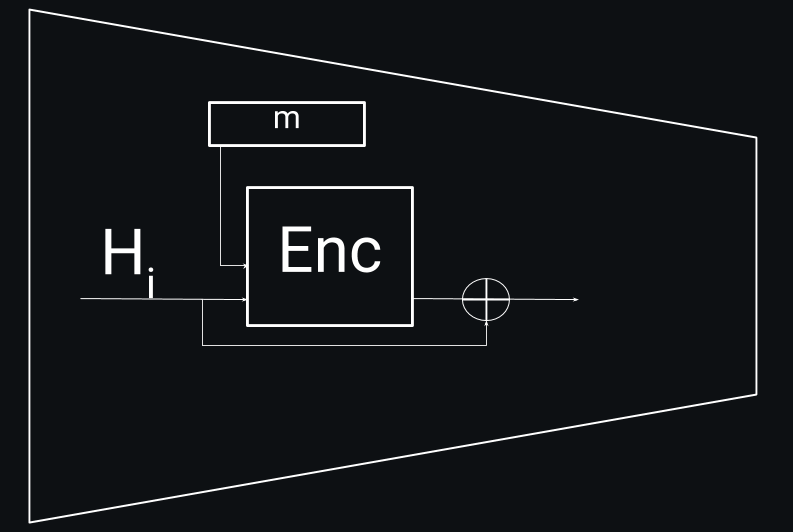
\includegraphics[width=\textwidth]{DaviesMeyerCompression}
\end{figure}
\end{column}
\end{columns}
\vspace{10pt}	

%Конструкция Davies-Meyer оптимальна при условии $\Enc$ \\ неотличима от случайной перестановки. 
\end{frame}

\begin{frame}{Альтернативные конструкции $h$}
\Large
\begin{columns}[T]
\begin{column}{0.5\textwidth}
{\color{Orange} Конструкция Davies-Meyer:}
\[
h(H, m) = \Enc(H, m)\oplus H
\]

{\color{Orange} Конструкция Miyaguchi–Preneel:}
\[
h(H, m) = \Enc(H, m)\oplus H \oplus m
\]

\vspace{10pt}	
ГОСТ  Р 34.11-2012 (Стрибог) использует Miyaguchi–Preneel.\\[7pt]
Другие комбинации $\Enc, H, m$ возможны, см. B. Preneel, R. Govaerts, J. Vandewalle. ``Hash functions based on block ciphers: a synthetic approach.''  \\[7pt]
Не все комбинации безопасны! \\[7pt]

\end{column}
\begin{column}{0.5\textwidth}
\begin{figure}
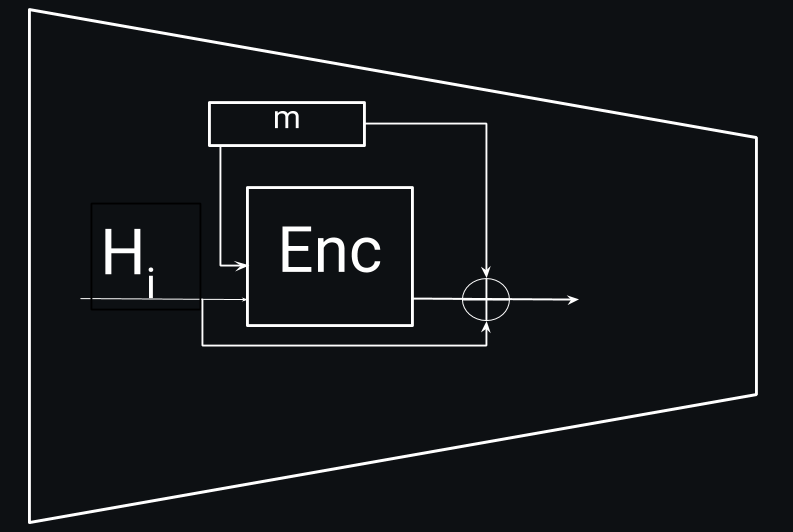
\includegraphics[width=\textwidth]{MiyaguchiPreneelCompression}

\vspace{30pt}	


\end{figure}
\end{column}
\end{columns}
\end{frame}

\begin{frame}
Часть IV \\ [10pt]
\begin{LARGE}
	
	\color{Orange}
	\Huge Где используются хэш-функции
	
\end{LARGE}
\end{frame}

\begin{frame}
\Large
\begin{itemize}
	\itemsep 10pt
	\item Построение MACa
	\item Протокол идентификации
	\item Доказательство работы (proof of work)
\end{itemize}
\end{frame}

\begin{frame}

\begin{LARGE}


\color{Orange}
1. Построение MACa

\end{LARGE}
\end{frame}

\begin{frame}{Построение MACa}
\Large
{\color{Orange} Задача:} из хэш-функции 
\[H: \{0,1\}^\star \rightarrow \{0,1\}^{\ell}\] построить функцию генерации МАСа 
\[S: \keyS \times \{0,1\}^\star \rightarrow \{0,1\}^{\ell}.\]

\vspace{20pt}

Основная сложность: хэш-функция -- бесключевой примитив. 

\end{frame}

\begin{frame}{Конструкция ``Two-key Nest''}
\Large
Для сообщения $M = (m_1, m_2)$ и $h: \{0,1\}^\ell \times \mesS \rightarrow  \{0,1\}^\ell $ -- функции компрессии
\[
S((k_1, k_2), M) = \Hash_{\text{NMAC}}(k_2 \; ||  \; \Hash_{\text{NMAC}}(k_1 \; || \; M)
\]

\begin{figure}
\hspace{-60pt}
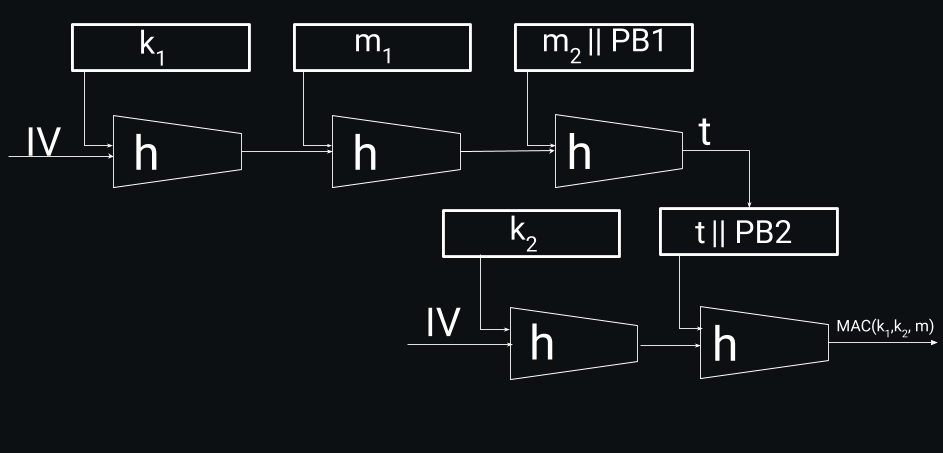
\includegraphics[scale=0.35]{TwoKeyNest}
\end{figure}
\vspace{-30pt}
{\color{Orange} Теорема:} Если $h(\cdot, )$ и $h(, \cdot)$ -- псевдослучайная функция, то \\ Two-key Nest -- безопасный MAC.

\end{frame}

\begin{frame}

\begin{LARGE}


\color{Orange}
2. Протокол идентификации

\end{LARGE}
\end{frame}

\begin{frame}{Протокол идентификации:  определение}
\Large
$\text{Id } = (\KeyGen, \textsf{P}, \textsf{V})$ -- интерактивный протокол, состоящий из 

\begin{itemize}
\itemsep 7pt
\item $\KeyGen(1^\lambda) \rightarrow (\vk, \sk)$ 
\item $\textsf{P}(\sk)$ -- Доказывающий (Prover)
\item $\textsf{V}(\vk) \rightarrow \{0,1\}$ -- Проверяющий (Verifier)
\end{itemize}

\vspace{10pt}

{\color{Orange} Корректность:} $\textsf{V}(\vk) \rightarrow 1$ при общении с $\textsf{\sk}$, где $\KeyGen(1^\lambda) = (\vk, \sk)$.

\vspace{10pt}

{\color{Orange} Безопасность:}
\begin{tabular}{c c c}
{\color{Orange} Челленджер $\mathcal{C}$ } & & {\color{Orange} $\mathcal{A}$ } \\ 
$\KeyGen(1^\lambda) \rightarrow (\vk, \sk)$ & $\xrightarrow{\vk}$ & \\[5pt]
& $\leftarrow$ & \\[-2pt]
& $\rightarrow$ & \\[2pt]

\end{tabular}
\vspace{10pt}

Выигрыш $\mathcal{A}$ --  $\mathcal{C}$ возвращает ``1'' (Accept). \\[5pt]

$\text{Id }$ -- безопасный Id-протокол относительно прямых атак,  \\ если $\forall $ ppt $\mathcal{A}$  вероятность выигрыша  $\negl(\lambda)$.

\end{frame}

\begin{frame}{Протокол парольной идентификации}
\Large
\[
\Hash: \{0,1\}^\star \rightarrow \{0,1\}^\ell - \text{ хэш-функция}
\]

\vspace{10pt}
\begin{center}
\begin{tabular}{c c c}
\multicolumn{3}{c}{$\KeyGen \rightarrow (\sk = pwd, \vk = \Hash(pwd))$}  \\[20pt] 
$\textsf{P}(pwd)$  & & $\textsf{V}(\vk)$  \\[5pt]
& $\xrightarrow{\quad pwd \quad }$ & \\
&  & $\Hash(pwd) == \vk \; ? \; 1 \; : \; 0 $
\end{tabular}
\end{center}

\vspace{10pt}

$\Hash$ -- криптографическая хэш-функция $\implies$ протокол  \\ $\text{Id} = (\KeyGen,\textsf{P}, \textsf{V} )$ безопасен относительно прямых атак.

\end{frame}


\begin{frame}{Протокол парольной идентификации}
\Large
\[
\Hash: \{0,1\}^\star \rightarrow \{0,1\}^\ell - \text{ хэш-функция}
\]

\vspace{10pt}
\begin{center}
\begin{tabular}{c c c}
\multicolumn{3}{c}{$\KeyGen \rightarrow (\sk = pwd, \vk = [\Hash(pwd, {\color{Orange}salt}), {\color{Orange}salt \xleftarrow{\$} S}])$}  \\[20pt] 
$\textsf{P}(pwd)$  & & $\textsf{V}(\vk = (h, {\color{Orange}salt}))$  \\[5pt]
& $\xrightarrow{\quad pwd \quad }$ & \\
&  & $\Hash(pwd, {\color{Orange}salt}) == h \; ? \; 1 \; : \; 0 $
\end{tabular}
\end{center}

\vspace{10pt}

$\Hash$ -- криптографическая хэш-функция $\implies$ протокол  \\ $\text{Id} = (\KeyGen,\textsf{P}, \textsf{V} )$ безопасен относительно прямых атак.

\end{frame}



\begin{frame}

\begin{LARGE}


\color{Orange}
3. Доказательство работы (proof of work)

\end{LARGE}
\end{frame}




\begin{frame}{Хэш-функция в  BitCoin}
\Large
Важный примитив в BitCoin: {\color{Orange} Proof of Work (PoW) / Доказательство работы} \\[10pt]
Интуиция: вычислительная мощность пользователя $\implies$ пользователь должен доказать это результатом вычислений \\
\vspace{15pt}
\begin{itemize}
\itemsep 1em
\item PoW предложен Dwork \& Naor (1992) как противодействие спаму
\item {\color{Orange} Идея:}  заставить пользователя решить пазл ``средней сложности''  (решение должно быть легко верифицировать)
\end{itemize}
\end{frame}

\begin{frame}{Хэш-функция в  BitCoin: конструкция PoW}

\large
Основной примитив: криптографическая хэш-функция  $\Hash:\{0,1\}^\star \rightarrow \{0,1\}^\ell$, сложность вычисления которой $T(\Hash)$.

\vspace{10pt}
%\begin{center}
\begin{tabular}{l c c c l}
& Алиса  & & Боб &  \\
& Доказывающий  & & Проверяющий &  \\[3pt]
& \multirow{5}{*}{
\includegraphics[scale=0.15]{Alice}} & & 
\multirow{5}{*}{
\includegraphics[scale=0.15]{Bob}} &  1. $x \in \{0,1\}^{\star}$   \\
&  & \Huge $\xleftarrow{\mkern5mu x \mkern5mu}$ & &  3. Проверить: \\ [2pt]
2. Выбрать $s \in \{0,1\}^\star$   & & &  & $\Hash(s||x)$  имеет $n$ 0ей?  \\[-6pt]
т.ч.\ $\Hash(s||x)$ & & \Huge $\xrightarrow{\mkern5mu s \mkern5mu}$  &  &  {\color{Orange}  Время: $T(\Hash) $}  \\
начинается с $n$ 0'ей & & &  &  \\[4pt]
{\color{Orange}  Время: $2^n T(\Hash) $} & & &  & 
\end{tabular}
%\end{center}

\vspace{15pt}
Для криптографической хэш-функции $\Hash$ Алиса не может найти $s$ \\ быстрее, чем перебором. Это атака на прообраз. 
\end{frame}



\end{document}